%%%%%%%%%%%%%%%%%%%%%%%%%%%%%%%%%%%%%%%%%%%%%%%%%%%%%%%%%%%%%%%%%%%%%%%%%%%%%%%%%%%%%%%%%%%%%%%
%% Credit: Initial version written by [Ivan C. Christov](http://christov.tmnt-lab.org),      %%
%% Purdue University.                                                                        %%
%% License: GPLv3 (see https://www.gnu.org/licenses/gpl-3.0.en.html)                         %%
%%%%%%%%%%%%%%%%%%%%%%%%%%%%%%%%%%%%%%%%%%%%%%%%%%%%%%%%%%%%%%%%%%%%%%%%%%%%%%%%%%%%%%%%%%%%%%%
\DocumentMetadata
    {
    % testphase = phase-I,    % tagging without paragraph tagging
    testphase  = phase-II,  % tagging with paragraph tagging
    % testphase  = phase-III, % tagging with paragraph sec, toc, blocks and more
    pdfversion = 2.0,       % pdfversion must be set here.
    pdfstandard=ua-2,       % pdfstandard can be set too
}
\documentclass[10pt,landscape]{article}

\usepackage[pdftitle={Lubrication Theory Summary Sheet}, pdflang=en-US]{hyperref}

\usepackage{amsmath}
\usepackage{pdflscape}
\usepackage{color}
\usepackage[margin=0.75in]{geometry}

\usepackage{fancyhdr}
\setlength{\headheight}{15.2pt}
\usepackage{totpages}

\fancyhead[L]{Purdue University, ME 50900}
\fancyhead[R]{Prof.\ Ivan C.\ Christov}
%\fancyfoot[C]{Page \thepage\ of \ref*{TotPages}}
\fancyfoot[C]{%
    \makebox[0pt][r]{Page\ }%
    \thepage
    \makebox[0pt][l]{\ of \ref*{TotPages}}%
}

\usepackage{accents}

% \DeclareMathOperator{\tr}{tr}

\usepackage[most]{tcolorbox}

\usepackage{tikz}
\usetikzlibrary{arrows.meta,calc}

\newtcolorbox{empheqboxed}{colback=gray!5,
    colframe=black,
    width=\textwidth,
    sharpish corners,
    top=-2mm, % default value 2mm
}

%--------------------------------------------------
% Colors
%--------------------------------------------------
%\definecolor{myred}{RGB}{180,20,20}
\definecolor{myred}{RGB}{204,7,30}
%\definecolor{mygreen}{RGB}{0,120,0}
\definecolor{mygreen}{RGB}{0,122,115}
%\definecolor{myblue}{RGB}{30,50,190}
\definecolor{myblue}{RGB}{0,87,184}

%\definecolor{onred}{RGB}{244,166,166}
\definecolor{onblue}{RGB}{166,209,245}
\definecolor{onyellow}{RGB}{255,245,157}

%--------------------------------------------------
% Macros
%--------------------------------------------------
\newcommand{\vvec}{\underline{v}}
\newcommand{\ex}{\underline{e}_x}
\newcommand{\ey}{\underline{e}_y}
\newcommand{\hly}[1]{\mbox{\colorbox{onyellow}{$\displaystyle #1$}}}
\newcommand{\hlb}[1]{\mbox{\colorbox{onblue}{$\displaystyle #1$}}}

% \setlength{\parindent}{0pt}
% \setlength{\fboxsep}{2pt}

\begin{document}

\thispagestyle{fancy}

\Large

%==================================================
% TWO-COLUMN LAYOUT
%==================================================
\noindent
\begin{minipage}[t]{0.45\textwidth}

    %------------------------------------------------
    % LEFT: Unidirectional Flow (exact)
    %------------------------------------------------
    \section*{\centering\fbox{Unidirectional flow \textcolor{red}{\textbf{(exact)}}}}

    \normalsize

    Velocity field kinematics:
    \[
       \vvec = v_x(y)\,\ex \qquad (~\Rightarrow \vvec\cdot\nabla\vvec = \underline{0}~)
    \]

    Basic equations:
    \begin{alignat*}{2}
        &\text{COM:} &\quad 0 &= 0 \\[7pt]
        &\text{COLM-}x\text{:} &\quad 0 &= -\frac{\partial p}{\partial x}
            + \mu\frac{\partial^2 v_x}{\partial y^2} \\[7pt]
        &\text{COLM-}y\text{:} &\quad 0 &= -\frac{\partial p}{\partial y}
    \end{alignat*}

    Typical 2D channel geometry (``combined Poiseuille--Couette flow''):
    %=== LEFT DIAGRAM ===
    % V_x arrow: attached to RIGHT END of top wall at (L, H)
    % No arrows above the wall — parabolic profile only inside channel
    \tagmcbegin{artifact}
    \begin{center}
    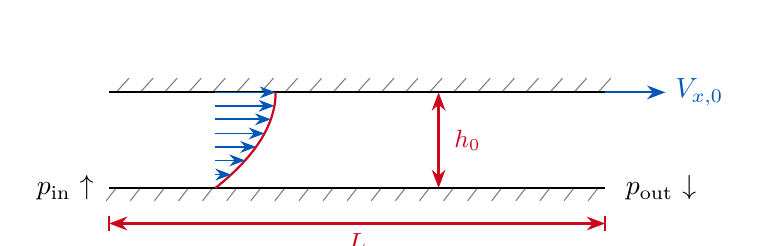
\begin{tikzpicture}[scale=0.9, >=Stealth]
        \def\L{7.0}
        \def\H{1.35}

        % -- Top wall: hatching first, black wall line drawn on top --
        \foreach \x in {0.10,0.44,...,6.90}
            \draw[gray,thin] (\x,\H) -- ++(0.18,0.20);
        \draw[thick,black] (0,\H) -- (\L,\H);

        % -- Bottom wall: hatching first, black wall line drawn on top --
        \foreach \x in {0.10,0.44,...,6.90}
            \draw[gray,thin] (\x,0) -- ++(-0.14,-0.18);
        \draw[thick,black] (0,0) -- (\L,0);

        % -- Poiseuille-Couette profile: V(y) = 0.85*(y/H)*(2-y/H)
        %    Scaled so V(H) = 0.85 = V_x arrow length (no-slip condition visible)

        % Red profile curve
        \draw[myred,thick]
            plot[domain=0:\H, samples=60, smooth]
            ({1.5 + 0.85*(\x/\H)*(2-\x/\H)}, \x);

        % Blue arrows — top arrow (y=H) exactly matches V_x arrow length
        \foreach \yy in {0.19,0.39,0.58,0.77,0.97,1.16,\H}{
            \pgfmathsetmacro{\vlen}{0.85*(\yy/\H)*(2-\yy/\H)}
            \draw[->,myblue,semithick] (1.5,\yy) -- ({1.5+\vlen},\yy);
        }

        % -- v_x: attached exactly to right end of top wall --
        \draw[->,myblue,thick] (\L,\H) -- (\L+0.85,\H)
            node[right] {$V_{x,0}$};

        % -- h_0 annotation: myred to match L arrow --
        \draw[<->,myred,thick] (4.65,0) -- (4.65,\H)
            node[midway,right=2pt,text=myred]{\small$h_0$};

        % -- p_in / p_out: aligned with bottom wall (y=0) --
        \node[left=2pt]  at (0, 0) {$p_\mathrm{in}~{\uparrow}$};
        \node[right=4pt] at (\L, 0) {$p_\mathrm{out}~{\downarrow}$};

        % -- L dimension line with | terminators --
        \draw[myred,thick] (0,-0.60) -- (0,-0.40);
        \draw[myred,thick] (\L,-0.60) -- (\L,-0.40);
        \draw[<->,myred,thick] (0,-0.50) -- (\L,-0.50)
            node[midway,below]{\small$L$};

    \end{tikzpicture}
    \end{center}
    \tagmcend

    \vspace{-2pt}

    Many other combinations of BCs possible!

    \vspace{2pt}

    Solution strategy:
    \begin{enumerate}
        \item $p$ is not a function of $y$ (from COLM-$y$)
        \item $v_x$ is not a function of $x$ (from kinematics)
        \item each term on RHS of COLM-$x$ must be constant:
        \begin{align*}
            % Pressure gradient: plain equality chain, NO misleading underbrace
            \frac{\partial p}{\partial x} &= \frac{dp}{dx} = \mathrm{const}. = \frac{p_\mathrm{in}-p_\mathrm{out}}{L} = -\hly{\frac{\Delta p}{L}}\\
            % Velocity solution: underbrace under (-dp/dx) only — correct placement
            v_x(y) &= \frac{h_0^2}{2\mu}
            \left(\hly{-\frac{dp}{dx}}\right)
            \left[\frac{y}{h_0} - \left(\frac{y}{h_0}\right)^{2}\right]
            + V_{x,0}\,\frac{y}{h_0}
        \end{align*}
        \item $Q = \int_0^{h_0} v_x(y)\,dy$ leads to flow rate--pressure \emph{drop} relation (\textbf{done!})
    \end{enumerate}

\end{minipage}%
%
\qquad
\vrule width 0.5pt
\qquad
%
\begin{minipage}[t]{0.53\textwidth}

    %------------------------------------------------
    % RIGHT: Lubrication Theory (approx)
    %------------------------------------------------
    \section*{\centering\fbox{Lubrication theory \textcolor{red}{\textbf{(approx)}}}}

    \normalsize

    Velocity field kinematics:
    \[
        \vvec = v_x(x,y)\,\ex + v_y(x,y)\,\ey \qquad (~\text{with}~\vvec\cdot\nabla\vvec \approx \underline{0}~)
    \]

    Basic equations:
    \begin{alignat*}{2}
        &\text{COM:} &\quad \frac{\partial v_x}{\partial x}
            + \frac{\partial v_y}{\partial y} &= 0 \\[7pt]
        &\text{COLM-}x\text{:} &\quad 0 &\approx
            -\frac{\partial p}{\partial x} + \mu\frac{\partial^2 v_x}{\partial y^2} \\[7pt]
        &\text{COLM-}y\text{:} &\quad 0 &\approx -\frac{\partial p}{\partial y}
    \end{alignat*}

    Typical 2D channel geometry:
    %=== RIGHT DIAGRAM ===
    % V_x arrow: attached to RIGHT END of top wall at (L, 0.86)
    % Streamlines: 5 plain arrows above wall, no V_x label there
    % h0<<L: label to the RIGHT of the vertical arrow
    % p_in / p_out: SAME y-height
    % Hatching positions recalculated to lie ON the Bezier curve
    \tagmcbegin{artifact}
    \begin{center}
    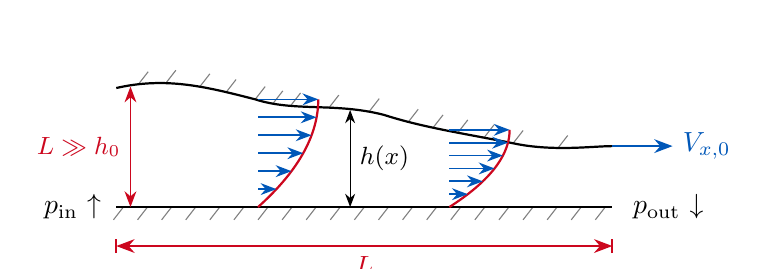
\begin{tikzpicture}[scale=0.9, >=Stealth]
        \def\L{7.0}
        \def\Hright{0.86}

        % -- Top wall: hatching first (x scaled ×1.4 from original), black curve on top --
        \foreach \xv/\yv in {
            0.31/1.73, 0.70/1.75, 1.18/1.70, 1.55/1.62, 1.96/1.52,
            2.21/1.46, 2.46/1.43, 3.00/1.40, 3.57/1.35, 4.12/1.20,
            4.47/1.12, 4.82/1.05, 5.19/0.98, 5.60/0.90, 6.23/0.83
        }{
            \draw[gray,thin] (\xv,\yv) -- ++(0.14,0.18);
        }
        \draw[thick,black]
            (0,1.68) .. controls (0.70,1.84) and (1.26,1.70) ..
            (1.96,1.52) .. controls (2.52,1.34) and (3.08,1.48) ..
            (3.78,1.30) .. controls (4.34,1.12) and (4.90,1.04) ..
            (5.60,0.90) .. controls (6.16,0.78) and (6.72,0.86) ..
            (\L,\Hright);

        % -- Bottom wall: hatching first, black wall on top --
        \foreach \x in {0.10,0.44,...,6.90}
            \draw[gray,thin] (\x,0) -- ++(-0.14,-0.18);
        \draw[thick,black] (0,0) -- (\L,0);

        % -- h0 annotation: arrow + "h0 << L" label to the right --
        \draw[<->,myred,semithick] (0.20,0) -- (0.20,1.7)
            node[midway,left=0pt]{\small$L \gg h_0$};

        % -- Velocity profile 1: x=2.0, local gap h(x1)=1.52 --
        %    Half-parabola: V(y) = 0.85*(y/h1)*(2-y/h1), top arrow = V_x
        \draw[myred,thick]
            plot[domain=0:1.52, samples=40, smooth]
            ({2.0 + 0.85*(\x/1.52)*(2-\x/1.52)}, \x);
        \foreach \kk in {1,2,3,4,5,6}{
            \pgfmathsetmacro{\yy}{\kk*1.52/6}
            \pgfmathsetmacro{\vlen}{0.85*(\yy/1.52)*(2-\yy/1.52)}
            \draw[->,myblue,semithick] (2.0,\yy) -- ({2.0+\vlen},\yy);
        }

        % -- h(x) annotation: placed between the two profiles --
        \draw[<->] (3.30,0) -- (3.30,1.37)
            node[midway,right=0pt]{\small$h(x)$};

        % -- Velocity profile 2: x=4.7, local gap h(x2)=1.09 --
        %    Same wall speed V_x at top; shorter profile since h(x2) < h(x1)
        \draw[myred,thick]
            plot[domain=0:1.09, samples=40, smooth]
            ({4.7 + 0.85*(\x/1.09)*(2-\x/1.09)}, \x);
        \foreach \kk in {1,2,3,4,5,6}{
            \pgfmathsetmacro{\yy}{\kk*1.09/6}
            \pgfmathsetmacro{\vlen}{0.85*(\yy/1.09)*(2-\yy/1.09)}
            \draw[->,myblue,semithick] (4.7,\yy) -- ({4.7+\vlen},\yy);
        }

        % -- v_x: attached to right end of top wall --
        \draw[->,myblue,thick] (\L,\Hright) -- (\L+0.85,\Hright)
            node[right] {$V_{x,0}$};

        % -- p_in / p_out: aligned with bottom wall --
        \node[left=2pt]  at (0, 0)    {$p_\mathrm{in}~{\uparrow}$};
        \node[right=4pt] at (\L, 0)   {$p_\mathrm{out}~{\downarrow}$};

        % -- Length arrow with | terminators at both ends --
        \draw[myred,thick] (0,-0.65) -- (0,-0.45);
        \draw[myred,thick] (\L,-0.65) -- (\L,-0.45);
        \draw[<->,myred,thick] (0,-0.55) -- (\L,-0.55)
            node[midway,below]{\small$L$};

    \end{tikzpicture}
    \end{center}
    \tagmcend

    \vspace{-2pt}

    Solution strategy:
    \begin{enumerate}
        \item $p$ is not a function of $y$ (COLM-$y$)
        \item $v_x$ \emph{is} a function of $x$; solve COLM-$y$ for $v_x$ in terms of $\hlb{\partial p/\partial x}$:
        \[
            v_x(x,y) = \frac{h(x)^2}{2\mu}
            \left(\hlb{-\dfrac{\partial p}{\partial x}}\right)
            \left[\frac{y}{h(x)} - \left(\frac{y}{h(x)}\right)^{2}\right]
            + V_{x,0}\,\frac{y}{h(x)}
        \]
        \item $Q = \int_0^{h(x)} v_x(x,y)\,dy$ leads to flow rate--pressure \emph{gradient} (\textbf{unknown!})
        \item write COM as $\partial v_y /\partial y = -\partial v_x/\partial x$
        \begin{enumerate}
            \item integrate over \emph{all} $y$ and use BCs to get ODE for $p(x)$
            \item integrate up to \emph{arbitrary} $y$ to find $v_y(x,y)$ (optional)
        \end{enumerate}
    \end{enumerate}

\end{minipage}

\end{document}
